% !TeX root=../main.tex
\setcounter{topnumber}{5}      % Increase number of floats at the top of the page
\setcounter{totalnumber}{5}    % Increase total number of floats on a page
\renewcommand{\floatpagefraction}{.8}  % Allow more of the page to be taken up by floats

\chapter{مروری بر مطالعات انجام شده}
%\thispagestyle{empty} 
\section{مقدمه}
در این فصل، پژوهش‌های پیشین در زمینه‌ی موتورهای صفحه‌ای مبتنی بر شناوری مغناطیسی (MLPM) با تمرکز بر ویژگی‌های اساسی آنان که به طور کلی در بخش‌های زیر دسته‌بندی شده‌اند، مورد بررسی قرار می‌گیرند. 

	\textbf{\textit{طراحی کنترلر}:}
	معرفی روش‌های کنترل کلاسیک و مدرن برای این سیستم‌ها و چگونگی بهبود پایداری و دقت حرکت.


در بخش‌های بعد، پژوهش‌های انجام‌شده بر اساس این ویژگی‌ها ارزیابی شده و مزایا و معایب هر روش مورد بررسی قرار می‌گیرد.

\section{معماری دستگاه‌های MLPM}
سیستم‌های شناوری مغناطیسی به دلیل ماهیت ناپایدارشان بدون استفاده از حلقه‌های کنترلی نمی‌توانند پایداری لازم را فراهم کنند. به همین دلیل، در تمامی ساختارهای پیشنهادی، از سیم‌پیچ‌های الکتریکی برای تولید میدان مغناطیسی با شدت کنترل ‌شده استفاده می‌شود. این سیم‌پیچ‌ها وظیفه دارند تا موقعیت جسم معلق را پایدار کرده و آن را در حالت مطلوب نگه ‌دارند.

در طراحی موتورهای صفحه‌ای، که از دو بخش ثابت
\LTRfootnote{Stator}
و متحرک
\LTRfootnote{Mover}
تشکیل شده‌اند، امکان تغییر در طراحی و محل قرارگیری آهنرباهای الکتریکی و دائمی وجود دارد. نیروی مغناطیسی وارد بر بخش متحرک می‌تواند به‌صورت جاذبه‌ای از بالا یا دافعه‌ای از پایین اعمال شود. با این حال، در موتورهای صفحه‌ای به دلیل لزوم کم بودن فاصله میان سیم‌پیچ‌ها و اجسام معلق، اعمال نیروی جاذبه‌ای از بالا امکان‌پذیر نیست. به همین دلیل، در تمامی طراحی‌ها، نیروی مغناطیسی دافعه‌ای از سمت پایین به بخش متحرک وارد می‌شود که امکان جابه‌جایی اجسامی که بر روی آنها قرار می‌گیرند را فراهم می‌کند.

با توجه به این موارد، طراحی های متفاوتی برای ساخت دستگاه‌های MLPM ارائه می‌شود که در ادامه بررسی یک مورد از آنان خواهیم پرداخت.


\subsection{‌آهنرباهای متحرک و سیم‌پیچ‌های ثابت}

معماری که برای طراحی دستگاه‌های MLPM ارائه شده است، شامل قرار دادن سیم‌پیچ‌ها در بخش استاتور و استفاده از آهنرباهای دائمی در بخش متحرک می‌باشد. این ساختار نوین که در بسیاری از پژوهش‌ها مورد استفاده قرار گرفته، مشکلات معماری‌های پیشین مانند محدودیت جابه‌جایی متحرک ناشی از اتصالات فیزیکی و چالش‌های خنک‌کاری سیم‌پیچ‌ها را برطرف کرده و منجر به بهبود عملکرد کلی سیستم شده است.

در پژوهش 
\cite{RN7}
استاتوری با چینش سیم‌پیچ‌ها مطابق با الگوی شاه‌ماهی
\LTRfootnote{Herringbone pattern}
طراحی و پیاده‌سازی شده است. این طراحی امکان اعمال نیروی مغناطیسی به دو آهنربای دیسکی تعبیه‌شده در بخش متحرک را فراهم کرده است که دقتی در حدود 1 درجه در زوایای حرکت و 1 میلی‌متر در موقعیت متحرک به دست آورده است
\cite{RN7}
. در ادامه این پژوهش، ساختاری جدید برای بخش متحرک ارائه شده که شامل 6 آهنربای دیسکی با چینش کروی و فواصل ثابت می‌باشد. این طراحی توانسته است چرخش آزادانه متحرک را حول سه محور ممکن سازد 
\cite{RN39}.
همچنین در پژوهش 
\cite{RN62}
نیز از این چینش سیم‌پیچ‌ها استفاده شده و مطابق با شبیه‌سازی‌های ارائه شده، مزیت آنان در ایجاد میدان مغناطیسی یکنواخت‌تر در نواحی کناری سیم‌پیچ‌ها نمایش داده شده است.

\section{طراحی کنترلر}
همان‌طور که پیش‌تر اشاره شد، سیستم‌های شناوری مغناطیسی ذاتاً ناپایدار هستند و برای دستیابی به پایداری، به کنترلری با عملکرد دقیق و خطای کم نیاز است. در پژوهش‌های مختلف، از کنترلرهای گوناگونی برای این سیستم‌ها بهره گرفته شده است؛ از جمله کنترلرهای کلاسیک نظیر PID، کنترلرهای مدرن مانند کنترل مبتنی بر پیش‌بینی مدل (MPC) و همچنین مدل‌های مبتنی بر هوش مصنوعی نظیر شبکه‌های بازگشتی GRU. در این بخش، به بررسی این کنترلرها و مقایسه‌ عملکرد آنها خواهیم پرداخت.
\subsection{کنترلر PID}

کنترل تناسبی-انتگرالی-مشتقی (PID) به عنوان یکی از پرکاربردترین و موثرترین کنترلرهای کلاسیک در سیستم‌های دینامیکی، گزینه‌ای مناسب برای کنترل سیستم‌های MLPM محسوب می‌شود. این کنترلر به دلیل سادگی در پیاده‌سازی، تنظیم دقیق و توانایی تنظیم خروجی سیستم بر اساس خطاهای ورودی، به‌طور گسترده در سیستم‌های مختلف استفاده شده است. برای کنترل سیستم‌های MLPM، به ازای هر درجه آزادی یک کنترلر PID طراحی و پیاده‌سازی می‌شود تا بتواند جریان الکتریکی سیم‌پیچ‌ها را تنظیم کرده و میدان مغناطیسی لازم برای ایجاد و حفظ موقعیت متحرک را تأمین کند.

در پژوهش‌های متعددی از کنترلر PID برای سیستم‌های MLPM بهره گرفته شده است. به عنوان مثال، در 
\cite{RN39,RN24}
از کنترلرهای PID ساده برای کنترل جریان سیم‌پیچ‌ها استفاده شده که وظیفه تنظیم میدان مغناطیسی و در نتیجه، کنترل موقعیت جسم متحرک را بر عهده دارند. علاوه بر این، در پژوهش
\cite{RN32}
، از دو کنترلر PID در یک ساختار دوگانه استفاده شده است. کنترلر اول برای جابه‌جایی‌های بلند و در مسافت‌های طولانی به کار رفته و جریان سیم‌پیچ‌های اصلی را تنظیم می‌کند، در حالی که کنترلر دوم برای حرکات دقیق کوتاه‌برد طراحی شده و کنترل جریان سیم‌پیچ‌های ثانویه را بر عهده دارد. این روش باعث بهینه‌سازی کنترل دقیق و بهبود دقت در حرکات کوتاه‌برد و جابه‌جایی‌های سریع می‌شود.
همچنین در سیستم MagTable، برای کنترل دقیق موقعیت آهنرباهای دائمی، از شش کنترلر PID به‌صورت همزمان استفاده شده است تا نیروی متوازن برای پایدارسازی موقعیت متحرک در چندین جهت فراهم شود 
\cite{RN8}
. این نوع طراحی و استفاده از کنترلرهای PID نشان می‌دهد که علی‌رغم محدودیت‌های موجود در کنترلرهای کلاسیک، این روش همچنان در بسیاری از سیستم‌های مغناطیسی پیچیده مانند MLPM کارایی بالایی دارد.

\begin{figure}[ht]
	\centering{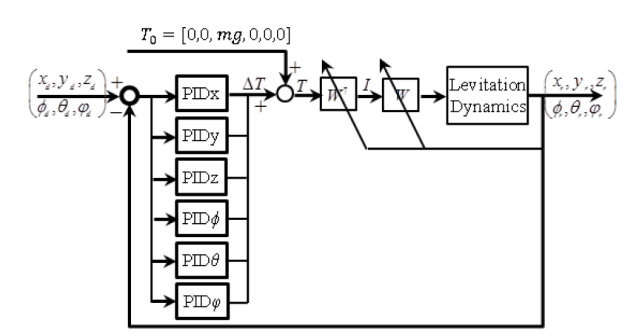
\includegraphics[width=0.5\textwidth]{PID_1}}
	\caption{کنترلر PID با 6 درجه آزادی
		\cite{RN8}}
	\label{fig:PID}
\end{figure}


\subsection{کنترلر مبتنی بر پیش‌بینی مدل MPC}
برای کنترل سیستم‌های MLPM اگر مدل سیستم به روش‌های تحلیلی و یا عددی به دست آمده و تخمین زده شده باشد، می‌توان از این مدل‌ها برای طراحی کنترلرهای پیشرفته‌تر با هدف پیش‌بینی رفتار سیستم و استفاده از آن به صورت پیش‌خور در حلقه‌ی کنترلی استفاده کرد. روش‌های تخمین مدل این سیستم‌ها در بخش‌های بعد مورد بررسی قرار می‌گیرد. در این بخش، کنترلرهای ارائه شده در پژوهش‌های دیگر ارائه می‌شود.
به دست آوردن معادلات دینامیکی سیستم و استفاده از آنها در پیش‌بینی روشی تحلیلی است که در 
\cite{RN55}
استفاده شده است و مدل کنترلی متشکل از بلوک‌های پس‌خور و پیش‌خور برای کنترل موقعیت آهنربا طراحی شده است. همچنین در 
\cite{RN62}
از یک جدول جستجو برای تعیین رفتار سیستم در نقاط مختلف فضا استفاده شده است که این جدول به عنوان پیش‌خور به مدل کنترلی داده می‌شود. در ادامه‌ی این پژوهش، با استفاده از روش‌های شناسایی سیستم، مدلی تقریبی برای رفتار سیستم در نظر گرفته شده است و با استفاده از این مدل برای پیش‌بینی رفتار سیستم‌ مدل MPC پیاده‌سازی شده است. پژوهش 
\cite{RN30}
با تمرکز بر ارائه‌ی یک مدل پیش‌بین، با استفاده از معادلات دینامیکی سیستم و همچنین روش‌پیش‌بینی حالت بی‌تاخیر، رفتار آینده‌ی سیستم را محاسبه می‌کند.
\begin{figure}[ht]
	\centering 
	\subfloat[\cite{RN55}]{
		\label{fig:MPC_1}
		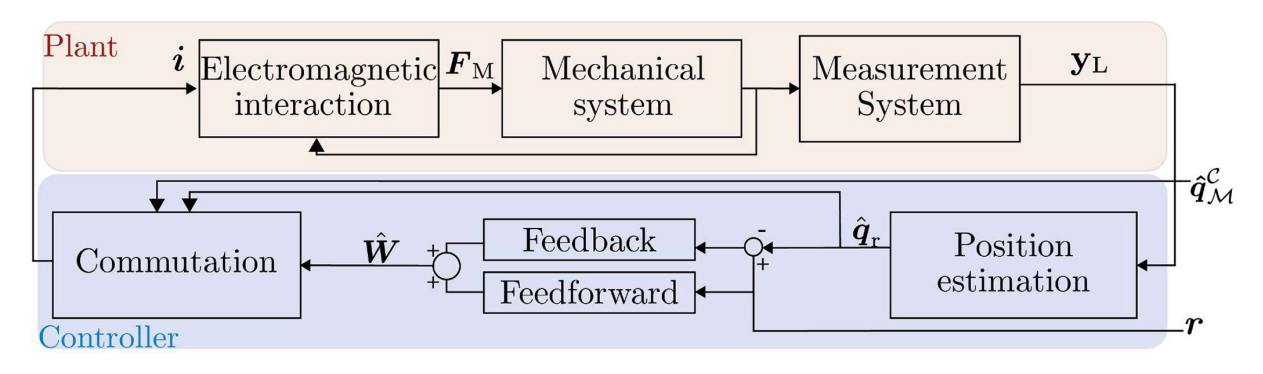
\includegraphics[width=0.45\textwidth]{MPC_1}}
	%\hspace{2mm}
	\subfloat[\cite{RN62}]{
		\label{fig:MPC_2}
		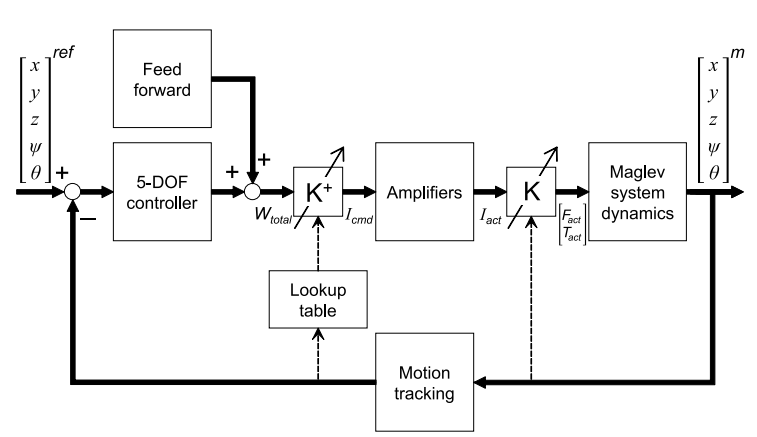
\includegraphics[width=0.45\textwidth]{MPC_2}}
	\\ % Newline to wrap the figures to the next row
	\subfloat[\cite{RN61}]{
		\label{fig:MPC_3}
		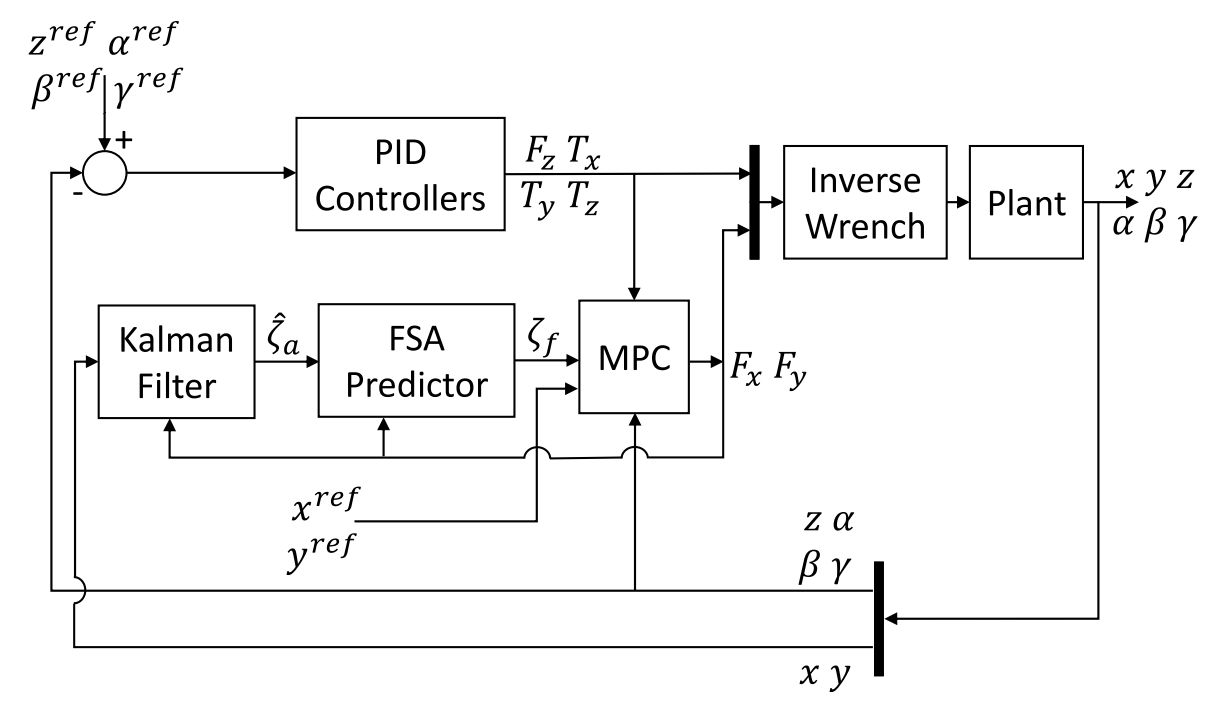
\includegraphics[width=0.45\textwidth]{MPC_3}}
	\subfloat[\cite{RN61}]{
		\label{fig:MPC_4}
		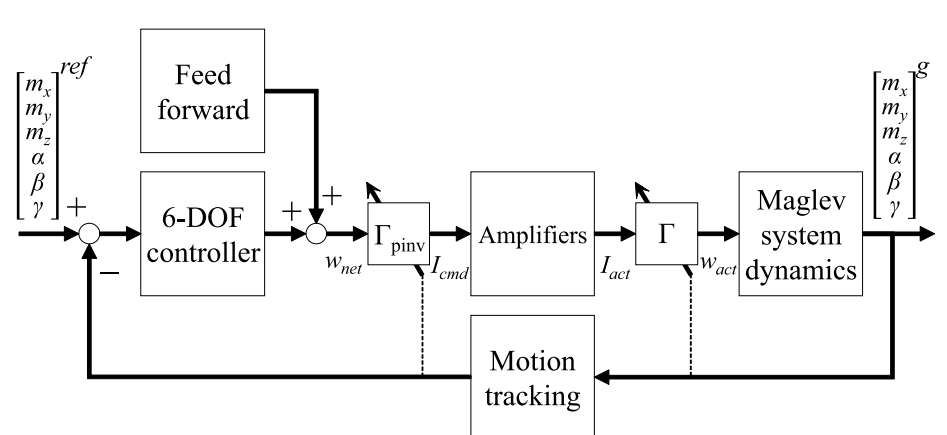
\includegraphics[width=0.45\textwidth]{MPC_4}}
	\caption{کنترلر MPC}
	\label{fig:MPC} %% label for entire figure
\end{figure}

\FloatBarrier

\subsection{کنترلر مبتنی بر هوش مصنوعی}

یکی از روش‌های نوین برای پیش‌بینی رفتار سیستم‌های پیچیده مانند MLPM، استفاده از مدل‌های هوش مصنوعی به‌ویژه شبکه‌های عصبی بازگشتی (RNN) است. این مدل‌ها با یادگیری دینامیک سیستم و ارتباط بین ورودی‌ها و خروجی‌ها، می‌توانند به‌طور مؤثری رفتار سیستم را در شرایط مختلف پیش‌بینی کنند. در این راستا، پژوهش
\cite{RN61}
از یک مدل بازگشتی GRU 
\LTRfootnote{Gated Recurrent Unit}
استفاده کرده است. این مدل بر اساس داده‌های جمع‌آوری‌شده از عملکرد دستگاه MLPM آموزش دیده و توانسته است با دقت بالا تغییرات دینامیکی سیستم و پاسخ آن به ورودی‌های گوناگون را پیش‌بینی کند. استفاده از GRU به دلیل توانایی آن در مدل‌سازی وابستگی‌های زمانی و در نظر گرفتن اطلاعات قبلی برای پیش‌بینی‌های دقیق‌تر، رویکردی مناسب در این پژوهش بوده است.(شکل 
\ref{fig:GRU}

\begin{figure}[H]
	\centering
	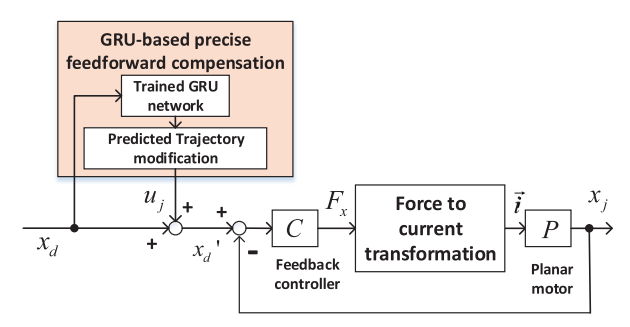
\includegraphics[width=0.5\textwidth]{GRU_1}
	\caption{کنترلر پیش‌خور GRU \cite{RN61}}
	\label{fig:GRU}
\end{figure}

